\chapter{The \smarthomeweather ontology}
\label{ch:smarthomeweather_ontology}


% TODO check if the things mentioned here are properly covered in the chapters referred

% TODO elaborate steps more?


The previous chapters cover all topics that require discussion before being able to build a new ontology from scratch: Chapter~\ref{ch:weather_data} discusses all details about weather data that is necessary and reasonable for the \smarthomeweather ontology, what data will be used and where to obtain it. Chapter~\ref{ch:existing_work} gives an overview about existing ontologies in the domain of weather data. As none of the existing ontologies being discussed fits the needs of a weather data ontology for smart homes, a new ontology is to be designed. Chapter~\ref{ch:development_approaches} analyses some of the most popular approaches for building ontologies from scratch. Among those, \methontology \cite{Methontology} is identified to be the best suitable approach.

Based on these insights, this chapter describes the process of designing the \smarthomeweather ontology in detail. The development process follows the steps proposed by \methontology as described in Chapter~\ref{sec:methontology}.

\section{Conventions}
\label{sec:ontology_conventions}

\begin{figure}
  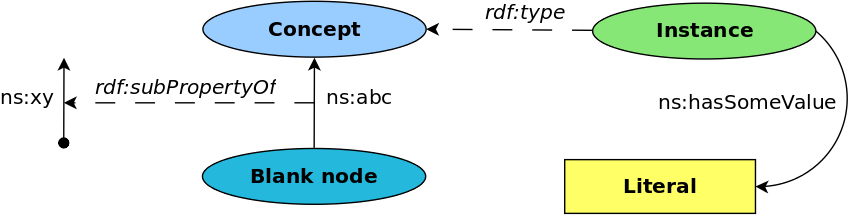
\includegraphics[width=\textwidth]{figures/diagrams/template.pdf}
  \caption{Example diagram}
  \label{fig:diagram_example}
\end{figure}

\definecolor{convention_color1}{HTML}{99CCFF}
\definecolor{convention_color2}{HTML}{87E776}
\definecolor{convention_color3}{HTML}{23B8DC}
\definecolor{convention_color4}{HTML}{FFFF66}
\definecolor{convention_color_bg4}{HTML}{AAAAAA}

All diagrams in this chapter showing parts of an ontology adhere to the following conventions, as seen in the example diagram shown in Figure~\ref{fig:diagram_example}. These conventions has already been adhered to in Chapter~\ref{ch:existing_work}:
\begin{itemize}
  \item \emph{Concepts} are drawn as ellipses filled with the color \texttt{\textcolor{convention_color1}{\#99CCFF}}.
  \item \emph{Instances} are drawn as ellipses filled with the color \texttt{\textcolor{convention_color2}{\#87E776}}.
  \item \emph{Blank nodes} are drawn as ellipses filled with the color \texttt{\textcolor{convention_color3}{\#23B8DC}}.
  \item \emph{Literals} are drawn as rectangles filled with the color \texttt{\colorbox{convention_color_bg4}{\textcolor{convention_color4}{\#FFFF66}}}.
  \item \emph{Properties in the \eacs{RDF}~\cite{RDF} and \eacs{RDFS}~\cite{RDFS} namespace} are drawn as dashed lines. Their caption is written in \emph{italics}.
  \item \emph{Properties in other namespaces} are drawn as solid lines. Their caption is \emph{not} written in \emph{italics}.
\end{itemize}

Every ontology should stick to a set of naming conventions that are explicitly stated~\cite{Ontology101}. The conventions for \smarthomeweather are as follows:

\begin{itemize}
  \item Two concepts, instances and/or properties may not have the same identifier as this is required by \eacs{OWL}~\cite{OWL}\footnote{Using one identifier for more than one concept, instance and properties is possible in \eacs{OWL} if an adequate number of namespaces is used. However, \smarthomeweather uses a single namespace.} and avoids confusion.
  \item Two identifiers may not use names that only differ in their capitalization. Using both \emph{Weather State} and \emph{weather state} in the name namespace is possible in \eacs{OWL}, but leads to confusion.
  \item Identifiers may only consist of upper and lower case \eacs{ASCII} letters (\emph{A} to \emph{Z} and \emph{a} to \emph{z}), numerical digits from \emph{0} to \emph{9} and spaces, i.e. all identifiers must match the regular expression \texttt{\textasciicircum[A-za-z0-9~]+\$}.
  \item \emph{Concepts} have an identifier that is in singular case and starts with an upper case letter. Typically a concept's identifier is a noun, e.g. \emph{Weather state} or \emph{Weather report}.
  \item \emph{Properties} have an identifier that starts with a lower case letter and starts with the prefix \emph{has} or \emph{belongs to}, followed by the name of the name of the concept which is the property's \emph{range}. The inverse property of a property having an identifier starting with \emph{has} has an identifier starting with \emph{belongs to}, followed by the inverse property's \emph{range}. As an alternative to the prefix \emph{belongs to}, the prefix \emph{is} in conjunction with the suffix \emph{of} and the inverse property's \emph{domain} may be used.
  
  E.g. the name of a property with the domain \emph{Weather report} and the range \emph{Weather state} has the name \emph{has weather state}. If \emph{has weather state} has an inverse property, it will have the name \emph{belongs to weather report} or \emph{is weather state of}.
\end{itemize}


\section{Specification}
\label{sec:ontology_specification}

\emph{Specification}, the first step proposed by \methontology, aims at creating an \emph{Ontology Requirements Specification Document} using natural language. It adheres to the approach discussed in Chapter~\ref{sec:methontology} and uses the document template taken presented in Section~\ref{subsec:methontology_specification}~\cite{ORSD}.

\vspace{1em}

% TODO ensure there are no problematic page breaks inside this box (e.g. between the headline 'Scope:' and the first bullet point)
\begin{mdframed}[linewidth=.6pt]
\setlength{\parindent}{0pt}
\vspace{.4cm}

\MakeUppercase{\textbf{Ontology Requirements Specification Document}}

\vspace{.6cm}

\textbf{Name}: \smarthomeweather

\vspace{.3cm}

\textbf{Purpose}: The ontology covers data about weather phenomena occurring at a certain location somewhere on Earth between the present and 24 hours in the future. Weather data will be acquired from both Internet services as well as from weather sensors mounted at the desired location. This weather data will enable a smart home system using \smarthomeweather to make decisions based on current and future weather conditions.

\vspace{.3cm}

\textbf{Scope}: The ontology has to cover a set of five core concepts from the domain of weather data:

\begin{itemize}
  \item \emph{weather phenomenon}: Represents a certain weather element. Relevant weather elements are \emph{temperature}, \emph{humidity}, \emph{dew point}, \emph{wind speed} and \emph{direction}, \emph{precipitation intensity} and \emph{probability}, \emph{atmospheric pressure}, \emph{cloud cover}, \emph{solar radiation}, and the \emph{sun's position}.
  \item \emph{Weather condition}: Overall state of the weather given by a simple verbal description: \emph{sun}, \emph{light clouds}, \emph{partly cloudy}, \emph{cloudy}, \emph{fog}, \emph{rain}, \emph{snow}, \emph{sleet}, \emph{thunder}.
  \item \emph{Weather state}: Summarises all weather phenomena for a certain time. 
  \item \emph{Weather report}: Summarises all data acquired at a certain time about the current weather or the weather some time in the future. Exactly one \emph{weather state} is linked to each \emph{weather report}.
  \item \emph{Weather report source}: Source where the data belonging to a \emph{weather report} has been obtained from (either an Internet weather service or a local weather sensor).
\end{itemize}

\vspace{.3cm}

\textbf{Implementation language}: The ontology is implemented in \emph{\eacs{OWL}~2}~\cite{OWL} using \protege~\cite{protege} and the \emph{Pellet reasoner}~\cite{pellet}.

\vspace{.3cm}

\textbf{Intended end-users}: End-users of the ontologies are inhabitants of smart homes. % TODO is the system itself the end-user?

\vspace{.3cm}

\textbf{Intended uses}: The ontology shall provide knowledge to ontology-based smart home systems about the current and future weather state in order to enable the system to make decisions based on that knowledge.

% TODO re-add this vspace?
\vspace{.3cm}

\textbf{Ontology requirements}:

\vspace{.3cm}

\setlength{\leftskip}{.5cm}

\textbf{Non-functional requirements}:

\begin{itemize}
  \item The ontology must adhere to the naming conventions presented in Section~\ref{sec:ontology_conventions} regarding the identifiers that may be used for classes, properties and individuals.
  \item The ontology must be documented thoroughly in order to make it easily reusable.
  \item The ontology must re-use existing ontologies wherever possible.
\end{itemize}

\textbf{Functional requirements}: The functional requirements are covered by the competency questions that the ontology shall be able to answer (see Section~\ref{sec:weather_information}):

\begin{itemize}
  \item What is the current weather situation?
  \item What will the weather situation be in one hour, in two hours, …, in 24 hours?
  \item What is the current temperature, humidity, wind speed, …?
  \item What will be the temperature, humidity, wind speed, … in one hour, in two hours, …, in 24 hours?
  \item What will be the minimum temperature, humidity, … over the next 24 hours? What about maximum values?
  \item Will the weather change? Will the temperature, humidity, … rise or fall?
  \item Does it rain? Will it rain in the next hours? Will it rain today?
  \item Will there be sunshine today? 
  \item Do we need to irrigate the garden?
  \item Will there be severe weather?
  \item Will temperature drop/stay below $0^\circ C$?
  \item When can we open windows and when do we have to keep them shut?
  \item When do we need sun protection?
  \item When will it outside be colder than inside the house? When will it be warmer?
\end{itemize}

\setlength{\leftskip}{0cm}

\vspace{.2cm}

\textbf{Pre-glossary of terms}: These are terms that can be extracted from the competency questions, in alphabetical order:

24 hours, airing, current weather, frost, future weather, humidity, humidity rise, humidity fall, irrigation, minimum, maximum, rain, room temperature, severe weather, sunshine, sun protection, temperature, temperature rise, temperature fall, weather change, wind speed.

\setlength{\leftskip}{0cm}

\end{mdframed}

\vspace{.5cm}

In the following sections, the \smarthomeweather ontology is built in a way to meet all above requirements, if possible. Section~\ref{sec:ontology_evaluation} evaluates if the resulting ontology fits the specification and which shortcomings the ontology comes with.

\section{Knowledge Acquisition}

The second step proposed by \methontology is \emph{Knowledge Acquisition}. All knowledge required to build the \smarthomeweather ontology is presented in Chapter~\ref{ch:existing_work} and Chapter~\ref{ch:weather_data}. These chapters discuss in detail:

\begin{itemize}
  \item Which weather data are relevant for smart homes?
  \item Which weather data are available from sensors (Section~\ref{sec:weather_sensors}) and Internet services (Section~\ref{sec:internet_services})? How can this data be acquired?
  \item Which data do not have any use for \smarthomeweather due to being too complicated or because they cannot be processed in an ontology in a useful way?
  \item What knowledge about weather in general is required to build an appropriate ontology~(cf. Chapter~\ref{ch:weather_data}?
\end{itemize}

Furthermore, Chapter~\ref{ch:existing_work} covers existing ontologies that cover the domain of weather data. An additional source of knowledge is available through works about weather in general, e.g. the \emph{Glossary of Meteorology}~\cite{GlossaryOfMeteorology} by the \emph{American Meteorological Society}~\cite{AMS}.

\section{Conceptualisation}
\label{sec:ontology_concept}

In the third step of \methontology, the \emph{Conceptualisation} step, the domain knowledge is structured into a conceptional model that describes the problem and its solution in terms of the domain vocabulary that has been identified in the \emph{Specification} process.

The starting point of \emph{Conceptualisation} is a complete \emph{Glossary of Terms} that covers all concepts, instances, attributes and binary relations that will form the ontology. Besides the glossary, this section covers \emph{Concept-classification trees} (Section~\ref{sec:concept_classification_trees}), \emph{Binary relationship diagrams} (Section~\ref{subsec:binary_relations_diagram}), \emph{Concept dictionaries} (Section~\ref{subsec:binary_relations_diagram}), \emph{Binary relations tables} (Section~\ref{subsec:binary_relations_table}), \emph{Instance attribute tables} (Section~\ref{subsec:binary_relations_table}) and \emph{Class attributes tables} (Section~\ref{subsec:class_attributes_table}). \emph{Constant tables}, \emph{Formal axiom tables} and \emph{Rules tables} have been omitted as the components described by these tables do not appear in \smarthomeweather.

In this section, only those deliverables are presented that are necessary to fully understand the structure of \smarthomeweather. All tables that have only been created for the sake of completeness can be found in Appendix~\ref{sec:appendix_conceptualisation}.

\subsection{Glossary of Terms}
\label{sec:ontology_glossary}

When describing the scope of \smarthomeweather, the \emph{Ontology Requirements Specification Document} in Section~\ref{sec:ontology_specification} mentions five top-level concepts (i.e. concepts that do not have a superclass except \emph{Thing} in \eacs{OWL}) of the ontology: \Egls{weather report}, \Egls{weather state}, \Egls{weather phenomenon}, and \Egls{weather condition}. All other concepts are sub-concepts of these five concepts.

In this section, only a list of terms is given; the complete \emph{Glossary of Terms} with short descriptions of each term can be found in Appendix~\ref{main}.

\paragraph{Concepts:}

Section~\ref{sec:weather_conclusion} presents the weather elements that are used in \smarthomeweather. In the ontology, weather elements are represented by concepts that are sub-concepts of \Egls{weather phenomenon}, e.g. there is a concept \Egls{temperature} for measurements of temperature, or \Egls{humidity} for measurements of relative humidity.

For all weather elements except \Egls{dew point}, categories are introduced in order to allow easy differentiation of weather observations by their respective measurement values. In the case of \Egls{temperature}, the sub-concepts differ from each other by the observed temperature values. The sub-concepts of \Egls{temperature} are \Egls{frost} (for an observed temperature value of below \SI{0}{\celsius}), \Egls{cold} (at least \SI{0}{\celsius} and less than \SI{10}{\celsius}), \Egls{below room temperature} (at least \SI{10}{\celsius} and less than \SI{20}{\celsius}), \Egls{room temperature} (at least \SI{20}{\celsius} and at most \SI{25}{\celsius}), \Egls{above room temperature} (more than \SI{25}{\celsius} and at most \SI{30}{\celsius}), and \Egls{heat} (more than \SI{30}{\celsius}). Refer to Section~\ref{sec:concept_classification_trees} for the concept-classification trees that result from this approach including the definitions of the respective sub-concepts.

A \egls{weather report} can encapsulate data either about the current weather or about the weather some time in the future which is specified by its \egls{start time}. Additionally, weather data can origin at a set of weather sensors or at an Internet weather service. To take this into account, a few sub-concepts of \egls{weather report} are introduced:

If the \egls{weather report} describes the current weather, it is a \Egls{current weather report}; if it describes the future weather, it is a \Egls{forecast weather report}. Depending on how far the \Egls{weather report}'s \egls{start time} lies ahead, it is a \Egls{short range weather report} (at most 3 hours in the future), a \Egls{medium range weather report} (more than 3 hours and less than 12 hours in the future) or a \Egls{long range weather report} (at least 12 hours in the future). Furthermore, there are sub-concepts of \egls{weather report}, each having a \egls{start time} of 1, 2, 3, 6, 9, 12, 15, 18, or 24 hours; these concepts are named \emph{Forecast 1 hour weather report}, \emph{Forecast 2 hours weather report} etc., respectively.

If the source of weather data is a \Egls{sensor source}, the corresponding \Egls{weather report} is a \Egls{weather report from sensor}; otherwise (if the source of weather data is a \Egls{service source}), it is a \Egls{weather report from service}.

A \Egls{weather report} that is both a \Egls{current weather report} and a \Egls{weather report from sensor} is a \Egls{current weather report from sensor}. A \Egls{weather report} that is both a \Egls{current weather report} and a \Egls{weather report from service} is a \Egls{current weather report from service}.

Several sub-concepts of \Egls{weather state} describe certain combinations of instances of \Egls{weather phenomenon} being associated with a \Egls{weather state}. These concepts are listed below; refer to the glossary in Appendix~\ref{main} for their definitions.

Thus, the concepts that can be found in \smarthomeweather are:
\begin{itemize}
  \item \Egls{weather condition}
  \item \Egls{weather phenomenon}:
    \begin{itemize}
      \item \Egls{atmospheric pressure}: \Egls{very low pressure}, \Egls{low pressure}, \Egls{average pressure}, \Egls{high pressure}, \Egls{very high pressure}
      \item \Egls{cloud cover}: \Egls{clear sky}, \Egls{partly cloudy}, \Egls{mostly cloudy}, \Egls{overcast}, \Egls{unknown cloud cover}.
      \item \Egls{dew point}.
      \item \Egls{humidity}: \Egls{very dry}, \Egls{dry}, \Egls{normal humidity}, \Egls{moist}, \Egls{very moist}.
      \item \Egls{precipitation}: \Egls{no rain}, \Egls{light rain}, \Egls{medium rain}, \Egls{heavy rain}, \Egls{extremely heavy rain}, \Egls{tropical storm rain}.
      \item \Egls{solar radiation}: \Egls{no radiation}, \Egls{low radiation}, \Egls{medium radiation}, \Egls{high radiation}, \Egls{very high radiation}.
      \item \Egls{sun position}: \Egls{day}, \Egls{solar twilight}, \Egls{sun below horizon}, \Egls{twilight}, \Egls{civil twilight}, \Egls{nautical twilight}, \Egls{astronomical twilight}, \Egls{night}, \Egls{sun from north}, \Egls{sun from east}, \Egls{sun from south}, \Egls{sun from west}.
      \item \Egls{temperature}: \Egls{frost}, \Egls{cold}, \Egls{below room temperature}, \Egls{room temperature}, \Egls{above room temperature}, \Egls{heat}.
      \item \Egls{wind}: \Egls{directional wind}, \Egls{north wind}, \Egls{east wind}, \Egls{south wind}, \Egls{west wind}, \Egls{calm}, \Egls{light wind}, \Egls{strong wind}, \Egls{storm}, \Egls{hurricane}.
    \end{itemize}
  \item \Egls{weather report}: \Egls{weather report from sensor}, \Egls{weather report from service}, \Egls{current weather report}, \Egls{current weather report from sensor}, \Egls{current weather report from service}, \Egls{forecast weather report}, \Egls{short range weather report}, \Egls{medium range weather report}, \Egls{long range weather report}, \emph{Forecast 1 hour weather report}, \emph{Forecast 2 hours weather report}, …, \emph{Forecast 24 hours weather report}
  \item \Egls{weather source}: \Egls{sensor source}, \Egls{service source}.
  \item \Egls{weather state}: \egls{airing weather}, \egls{calm weather}, \egls{clear weather}, \egls{cloudy weather}, \egls{cold weather}, \egls{dry weather}, \egls{fair weather}, \egls{hot weather}, \egls{moist weather}, \egls{no rain weather}, \egls{pleasant temperature weather}, \egls{rainy weather}, \egls{severe weather}, \egls{sun protection weather}, \egls{thunderstorm}, \egls{very rainy weather}, \egls{windy weather}
\end{itemize}

\paragraph{Relations:}

Instances of the concepts are associated to each other with binary relations, which are:

\begin{itemize}
  \item \egls{has source} and \egls{is source of} which connect instances of \Egls{weather report} and \Egls{weather source}.
  \item \egls{has weather state} and \egls{belongs to weather report} which connect instances of \Egls{weather report} and \Egls{weather state}.
  \item \egls{has condition} which connects instances of \Egls{weather state} and \Egls{weather condition}.
  \item \egls{has weather phenomenon} and \egls{belongs to state} which connect instances of \Egls{weather state} and \Egls{weather phenomenon}.
  \item \egls{has previous weather state} and \egls{has next weather state} which connect two instances of \Egls{weather state}.
\end{itemize}

The following relations link instances of concepts from other ontologies than \smarthomeweather to instances of concepts inside the ontology: \egls{has start time}, \egls{has end time}, \egls{has observation time}, and \egls{location}.

The only data property in \smarthomeweather is \egls{has priority} which specifies an integer value indicating which \Egls{weather report} for a certain period of time is to be preferred over another \Egls{weather report} for the same period of time.

\paragraph{Individuals:}

The only predefined individuals are instances of the concept \Egls{weather condition}; they represent the overall state of the weather for a certain \Egls{weather state}. These individuals are: \emph{cloud}, \emph{fog}, \emph{light clouds}, \emph{partly cloudy}, \emph{rain}, \emph{sleet}, \emph{snow}, \emph{sun}, and \emph{thunder}.

\subsection{Concept-classification trees}
\label{sec:concept_classification_trees}

As stated in Section~\ref{sec:ontology_glossary}, there are five top-level concepts; all other concepts are sub-concepts to these top-level concepts. As a consequence, each of these concepts becomes root of a tree of concepts. These \emph{Concept-classification trees} are presented in this section.

A \Egls{weather condition} does not have any sub-concepts. Hence, its classification tree which is shown in Figure~\ref{fig:tree_weather_condition} consists of only one element.

\begin{figure}
  \centering
  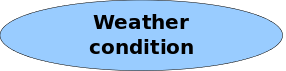
\includegraphics[width=.3\textwidth]{figures/diagrams/weather-condition.pdf}
  \caption{Concept-classification tree for \Egls{weather condition}}
  \label{fig:tree_weather_condition}
\end{figure}

A \Egls{weather phenomenon} represents a certain weather element. Every specific weather element is a sub-concept of \Egls{weather phenomenon}; the evolving tree is shown in Figure~\ref{fig:tree_weather_phenomenon}. For sake of clarity, this tree is broken up to several diagrams; all sub-concepts of sub-concepts of \Egls{weather phenomenon} are not shown in Figure~\ref{fig:tree_weather_phenomenon}. There is a separate diagram for each sub-concept of \Egls{weather phenomenon}:

\begin{figure}
  \centering
  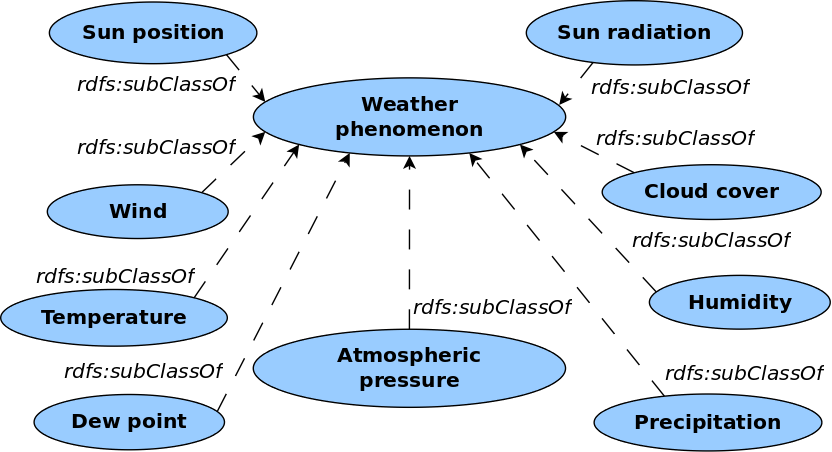
\includegraphics[width=.8\textwidth]{figures/diagrams/weather-phenomenon.pdf}
  \caption{Concept-classification tree for \Egls{weather phenomenon}}
  \label{fig:tree_weather_phenomenon}
\end{figure}

\begin{itemize}
  \item \Egls{atmospheric pressure} (Figure~\ref{fig:tree_atmospheric_pressure}): Depending on the pressure value, an instance of \Egls{atmospheric pressure} is an instance of exactly one of its sub-concepts: \Egls{very low pressure} (pressure value below \SI{998}{\hecto\pascal}), \Egls{low pressure} (at least \SI{998}{\hecto\pascal} and less than \SI{1008}{\hecto\pascal}), \Egls{average pressure} (at least \SI{1008}{\hecto\pascal} and less than \SI{1018}{\hecto\pascal}), \Egls{high pressure} (at least \SI{1018}{\hecto\pascal} and less than \SI{1028}{\hecto\pascal}), and \Egls{very high pressure} (at least \SI{1028}{\hecto\pascal}).
  
  \begin{figure}
    \centering
    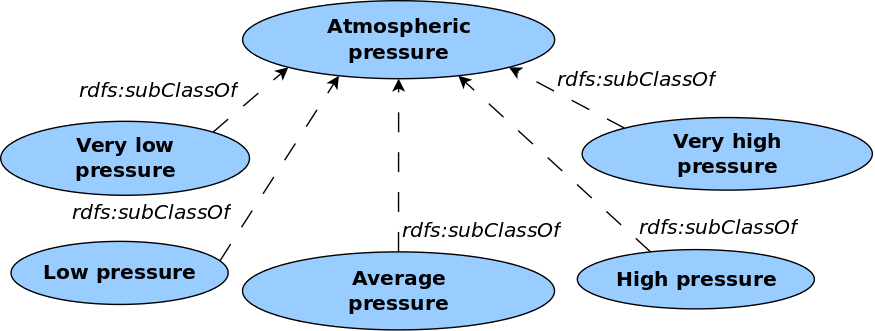
\includegraphics[width=.8\textwidth]{figures/diagrams/atmospheric-pressure.pdf}
    \caption{Concept-classification tree for \Egls{atmospheric pressure}}
    \label{fig:tree_atmospheric_pressure}
  \end{figure}

  % TODO definition of "okta"
  \item \Egls{cloud cover} (Figure~\ref{fig:tree_cloud_cover}): The sub-concepts of \Egls{cloud cover} are defined using different cloud coverage values: \Egls{clear sky} (cloud coverage of \num{0}$\:$\emph{okta}), \Egls{partly cloudy} (\num{1}$\:$\emph{okta} to \num{4}$\:$\emph{okta}), \Egls{mostly cloudy} (\num{5}$\:$\emph{okta} to \num{7}$\:$\emph{okta}), \Egls{overcast} (\num{8}$\:$\emph{okta}) and \Egls{unknown cloud cover} (\num{9}$\:$\emph{okta}).
  
  \begin{figure}
    \centering
    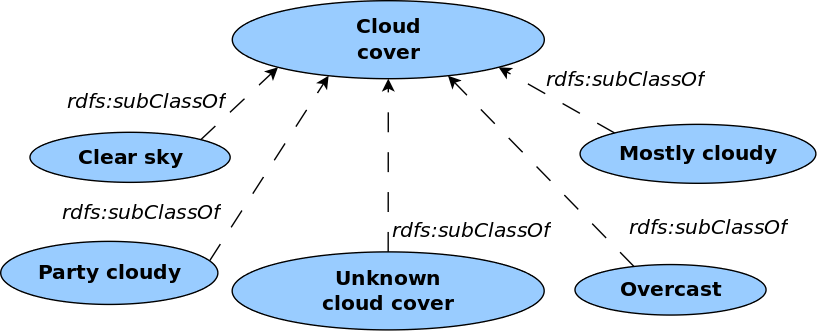
\includegraphics[width=.8\textwidth]{figures/diagrams/cloud-cover.pdf}
    \caption{Concept-classification tree for \Egls{cloud cover}}
    \label{fig:tree_cloud_cover}
  \end{figure}

  \item \Egls{humidity} (Figure~\ref{fig:tree_humidity}): The sub-concepts of \Egls{humidity} are \Egls{very dry} (value of relative humidity of less than \num{30} percent), \Egls{dry} (at least \num{30} percent and less than \num{40} percent), \Egls{normal humidity} (at least \num{40} percent and at most \num{70} percent), \Egls{moist} (more than \num{70} percent and at most \num{80} percent), and \Egls{very moist} (more than \num{80} percent).
  
  \begin{figure}
    \centering
    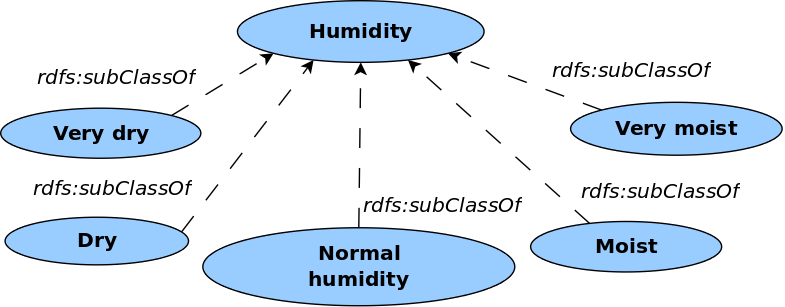
\includegraphics[width=.8\textwidth]{figures/diagrams/humidity.pdf}
    \caption{Concept-classification tree for \Egls{humidity}}
    \label{fig:tree_humidity}
  \end{figure}

  \item \Egls{precipitation} (Figure~\ref{fig:tree_precipitation}): The sub-concepts of \Egls{precipitation} are \Egls{no rain} (precipitation intensity of \SI{0}{\milli\metre\per\hour}), \Egls{light rain} (precipitation intensity of more than \SI{0}{\milli\metre\per\hour} and at most \SI{5}{\milli\metre\per\hour}), \Egls{medium rain} (precipitation intensity of more than \SI{5}{\milli\metre\per\hour} and at most \SI{20}{\milli\metre\per\hour}), \Egls{heavy rain} (precipitation intensity of more than \SI{20}{\milli\metre\per\hour} and at most \SI{50}{\milli\metre\per\hour}), \Egls{extremely heavy rain} (precipitation intensity of more than \SI{50}{\milli\metre\per\hour} and at most \SI{100}{\milli\metre\per\hour}), and \Egls{tropical storm rain} (precipitation intensity of more than \SI{100}{\milli\metre\per\hour}). For \Egls{no rain}, the precipitation probability is \num{0}; for the other sub-concepts, the precipitation probability is greater than \num{0}.
  
  \begin{figure}
    \centering
    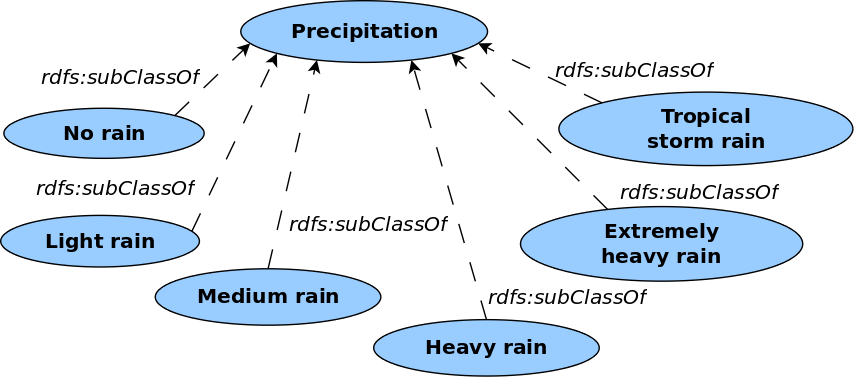
\includegraphics[width=.8\textwidth]{figures/diagrams/precipitation.pdf}
    \caption{Concept-classification tree for \Egls{precipitation}}
    \label{fig:tree_precipitation}
  \end{figure}
  
  \item \Egls{solar radiation} (Figure~\ref{fig:tree_solar_radiation}): In this case, the sub-concepts are \Egls{no radiation} (solar radiation value of \SI{0}{\watt\per\square\meter}), \Egls{low radiation} (solar radiation value of more than \SI{0}{\watt\per\square\meter} and less than \SI{250}{\watt\per\square\meter}), \Egls{medium radiation} (solar radiation value of more than \SI{250}{\watt\per\square\meter} and less than \SI{500}{\watt\per\square\meter}), \Egls{high radiation} (solar radiation value of more than \SI{500}{\watt\per\square\meter} and less than \SI{750}{\watt\per\square\meter}), \Egls{very high radiation} (solar radiation value of more than \SI{750}{\watt\per\square\meter}).
  
  \begin{figure}
    \centering
    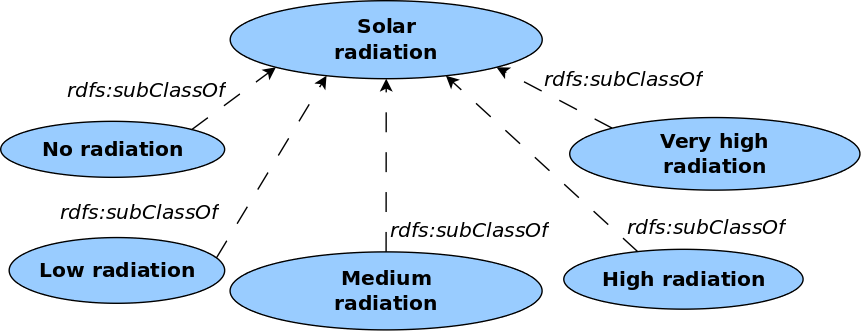
\includegraphics[width=.8\textwidth]{figures/diagrams/solar-radiation.pdf}
    \caption{Concept-classification tree for \Egls{solar radiation}}
    \label{fig:tree_solar_radiation}
  \end{figure}

  \item \Egls{sun position} (Figure~\ref{fig:tree_sun_position}): There are sub-concepts that are defined depending on the sun's azimuth angle, while others are defined depending on the sun's elevation above horizon:
    \begin{itemize}
      \item Those depending on the azimuth angle are \Egls{sun from north} (azimuth angle of at least \SI{0}{\degree} and at most \SI{45}{\degree} or of more than \SI{315}{\degree} and less than \SI{360}{\degree}), \Egls{sun from east} (azimuth angle of more than \SI{45}{\degree} and at most \SI{135}{\degree}), \Egls{sun from south} (azimuth angle of more than \SI{135}{\degree} and at most \SI{225}{\degree}), and \Egls{sun from east} (azimuth angle of more than \SI{225}{\degree} and at most \SI{315}{\degree}).
      
      \item The sub-concepts defined via the elevation angle are \Egls{day} (elevation angle of at least \SI{0}{\degree} and at most \SI{90}{\degree}), \Egls{solar twilight} (elevation angle of at least \SI{0}{\degree} and less than \SI{6}{\degree}), \Egls{sun below horizon} (elevation angle of at least \SI{-90}{\degree} and less than \SI{0}{\degree}), \Egls{twilight} (elevation angle of at least \SI{-18}{\degree} and less than \SI{0}{\degree}), \Egls{civil twilight} (elevation angle of at least \SI{-6}{\degree} and less than \SI{0}{\degree}), \Egls{nautical twilight} (elevation angle of at least \SI{-12}{\degree} and less than \SI{-6}{\degree}), \Egls{astronomical twilight} (elevation angle of at least \SI{-18}{\degree} and less than \SI{-12}{\degree}), and \Egls{night} (elevation angle of at least \SI{-90}{\degree} and less than \SI{-18}{\degree}). Refer to the \emph{Glossary of Meteorology} for the definitions of the different states of twilight~\cite{GlossaryOfMeteorology}.
    \end{itemize}
  
  \begin{figure}
    \centering
    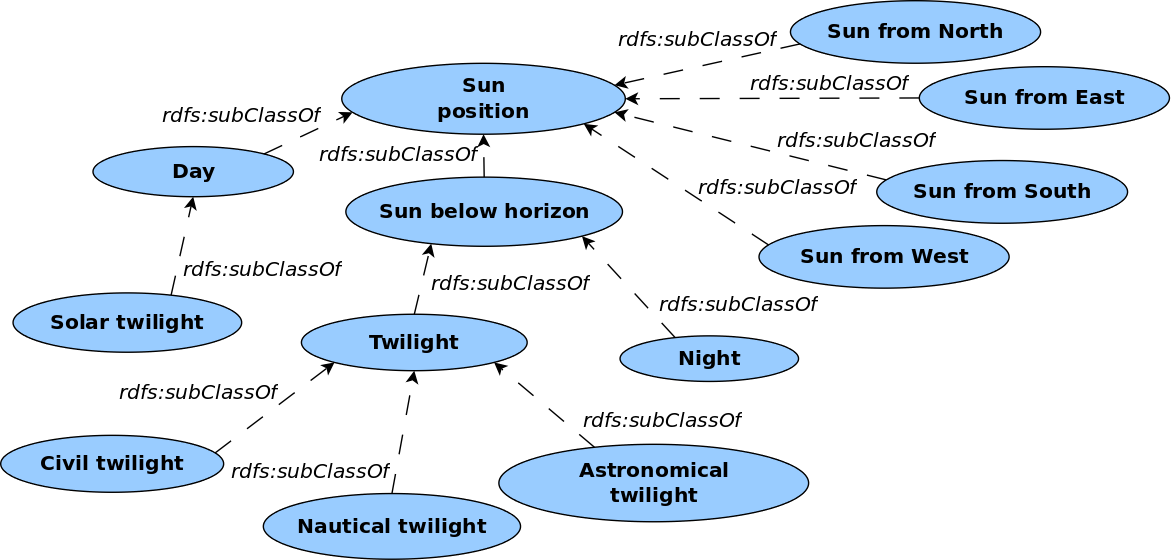
\includegraphics[width=\textwidth]{figures/diagrams/sun-position.pdf}
    \caption{Concept-classification tree for \Egls{sun position}}
    \label{fig:tree_sun_position}
  \end{figure}

  \item \Egls{temperature} (Figure~\ref{fig:tree_temperature}): The sub-concepts of \Egls{temperature} are \Egls{frost} (temperature value below \SI{0}{\celsius}), \Egls{cold} (at least \SI{0}{\celsius} and less than \SI{10}{\celsius}), \Egls{below room temperature} (at least \SI{10}{\celsius} and less than \SI{20}{\celsius}), \Egls{room temperature} (at least \SI{20}{\celsius} and at most \SI{25}{\celsius}), \Egls{above room temperature} (more than \SI{25}{\celsius} and at most \SI{30}{\celsius}), and \Egls{heat} (more than \SI{30}{\celsius}).
  
  \begin{figure}
    \centering
    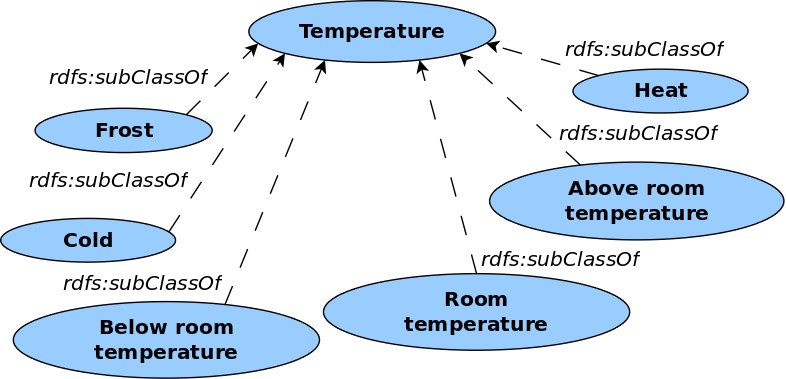
\includegraphics[width=.8\textwidth]{figures/diagrams/temperature.pdf}
    \caption{Concept-classification tree for \Egls{temperature}}
    \label{fig:tree_temperature}
  \end{figure}

  \item \Egls{wind} (Figure~\ref{fig:tree_wind}): As for \Egls{sun position}, there are two types of sub-concepts of \Egls{wind} -- those defined by the wind speed and those defined by the wind direction:
    \begin{itemize}
      \item If an instance of \Egls{wind} has the property \egls{has wind direction}, it is defined to be an instance of \Egls{directional wind}. This concept in turn has four sub-concepts: \Egls{north wind} (wind direction of at least \SI{0}{\degree} and less than \SI{45}{\degree} or of at least \SI{315}{\degree} and less than \SI{360}{\degree}), \Egls{east wind} (at least \SI{45}{\degree} and less than \SI{135}{\degree}), \Egls{south wind} (at least \SI{135}{\degree} and less than \SI{225}{\degree}), and \Egls{east wind} (at least \SI{225}{\degree} and less than \SI{315}{\degree}).
      
      \item Depending on the wind speed, there are the sub-concepts \egls{calm} (wind speed of at least \SI{0}{\kilo\metre\per\hour} and less than \SI{1}{\kilo\metre\per\hour}), \egls{light wind} (at least \SI{1}{\kilo\metre\per\hour} and less than \SI{10}{\kilo\metre\per\hour}), \egls{strong wind} (at least \SI{10}{\kilo\metre\per\hour} and less than \SI{20}{\kilo\metre\per\hour}), \egls{storm} (at least \SI{20}{\kilo\metre\per\hour}), and \egls{hurricane} (at least \SI{32}{\kilo\metre\per\hour}).
      
    \end{itemize}
    
  \begin{figure}
    \centering
    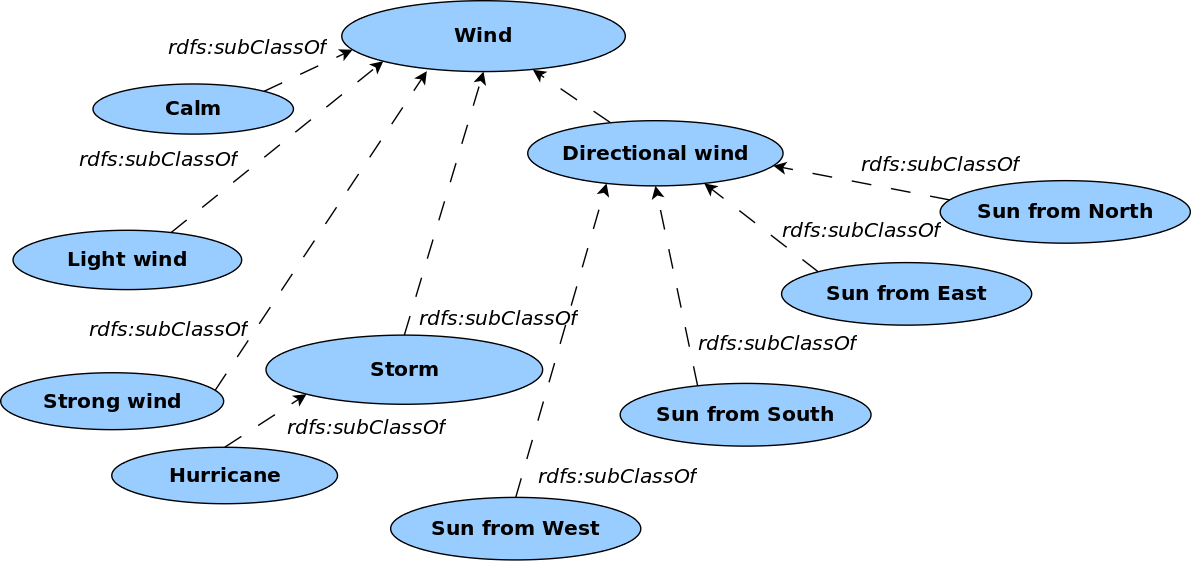
\includegraphics[width=\textwidth]{figures/diagrams/wind.pdf}
    \caption{Concept-classification tree for \Egls{wind}}
    \label{fig:tree_wind}
  \end{figure}

\end{itemize}

There is no separate diagram for \Egls{dew point} as that concept does not have any sub-concepts; hence its concept-classification tree consists of a single node.

Refer to Section~\ref{sec:appendix_conceptualisation} in the appendix for a tabular display of the sub-concepts of \Egls{weather phenomenon}.

A \Egls{weather report} has two attributes that define its main characteristics: \egls{has start time} and \egls{has source}. As discussed in Section~\ref{sec:ontology_glossary}, a number of sub-concepts is defined in order to reflect different values of these two attributes. The resulting concept-classification tree is shown in Figure~\ref{fig:tree_weather_report}.

\begin{figure}
  \centering
  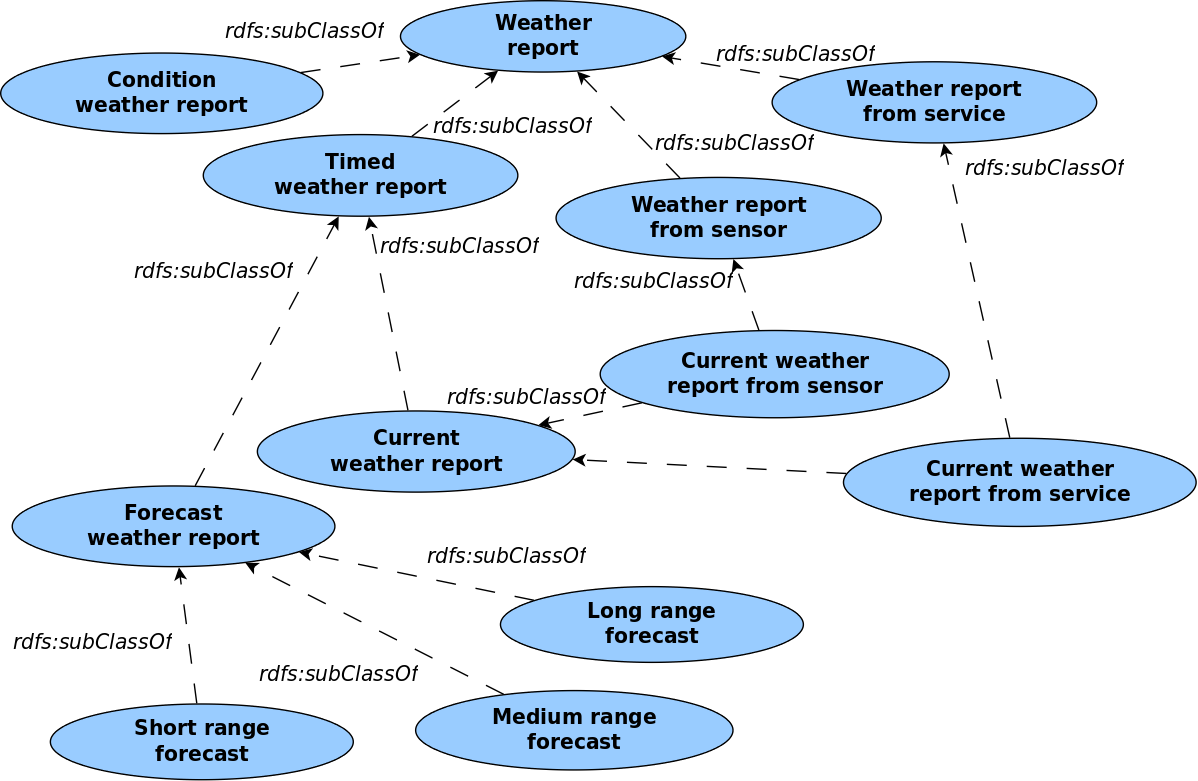
\includegraphics[width=\textwidth]{figures/diagrams/weather-report.pdf}
  \caption{Concept-classification tree for \Egls{weather report}}
  \label{fig:tree_weather_report}
\end{figure}

The concepts \Egls{short range weather report}, \Egls{medium range weather report} and \Egls{long range weather report} each do have sub-concepts which have been omitted from the above diagram for clarity. These sub-concepts are:
\begin{itemize}
  \item \Egls{short range weather report}: \emph{Forecast 1 hour weather report}, \emph{Forecast 2 hours weather report} and \emph{Forecast 3 hours weather report} for weather reports describing the weather in one, two and three hours, respectively.
  \item \Egls{medium range weather report}: \emph{Forecast 6 hour weather report} and \emph{Forecast 9 hours weather report} for weather reports describing the weather in 6 and 9 hours, respectively.
  \item \Egls{long range weather report}: \emph{Forecast 12 hour weather report}, \emph{Forecast 15 hours weather report}, \emph{Forecast 18 hours weather report}, \emph{Forecast 21 hours weather report} and \emph{Forecast 24 hours weather report} for weather reports describing the weather in 12, 15, 18, 21 and 24 hours, respectively.
\end{itemize}

A \Egls{weather source} can either be a \Egls{sensor source} or a \Egls{service source} (see Figure~\ref{fig:tree_weather_source}).

\begin{figure}
  \centering
  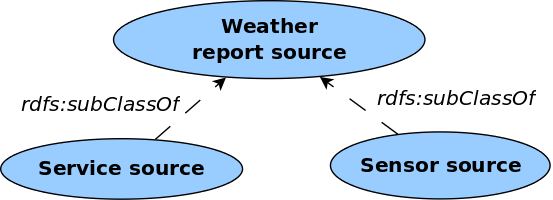
\includegraphics[width=.5\textwidth]{figures/diagrams/weather-report-source.pdf}
  \caption{Concept-classification tree for \Egls{weather source}}
  \label{fig:tree_weather_source}
\end{figure}

A \Egls{weather state} represents the set of weather phenomena that belong to a certain \Egls{weather report}. In order to emphasise certain combinations of instances of \Egls{weather phenomenon} being linked to the same instance of \Egls{weather state}, several sub-concepts of \Egls{weather state} are introduced (see Section~\ref{sec:ontology_glossary}). The resulting tree is seen in Figure~\ref{fig:tree_weather_state}.

\begin{figure}
  \centering
  % TODO description for this figure
  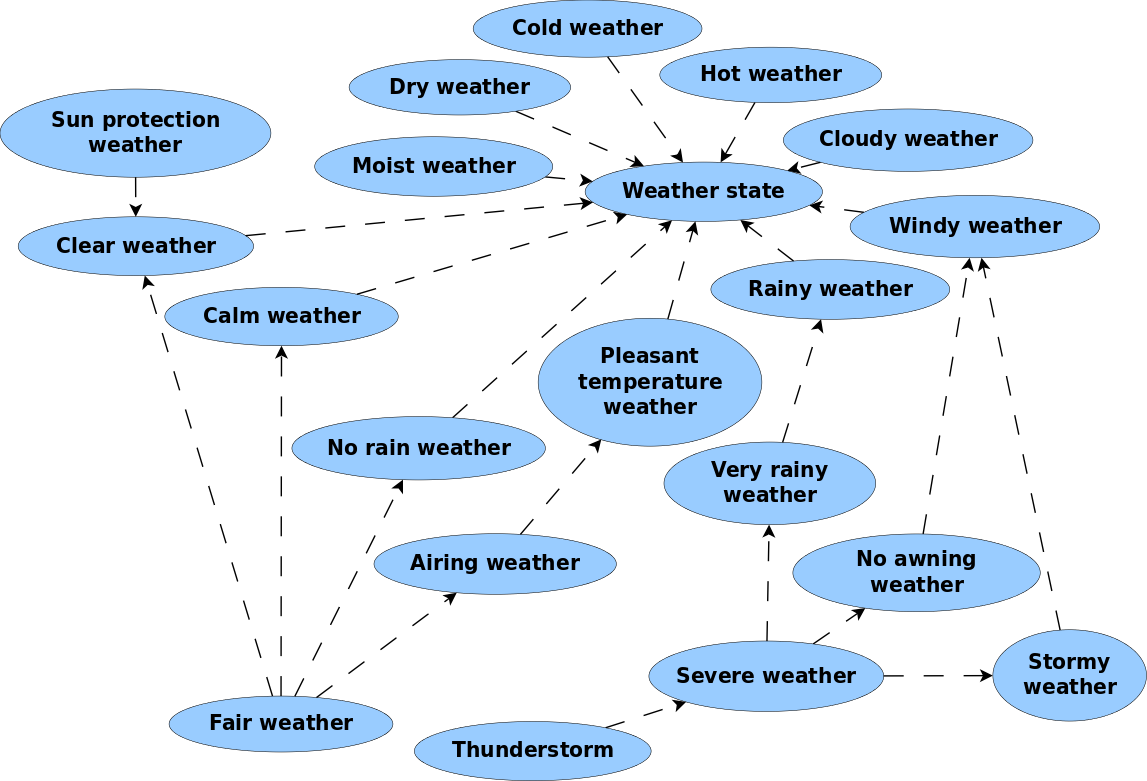
\includegraphics[width=\textwidth]{figures/diagrams/weather-state.pdf}
  \caption{Concept-classification tree for \Egls{weather state}. All properties are of type \emph{rdfs:subClassOf}}
  \label{fig:tree_weather_state}
\end{figure}

\subsection{Binary relations diagram}
\label{subsec:binary_relations_diagram}

The purpose of a \emph{Binary relations diagram} is to present all binary relations between concepts in the ontology (see Figure~\ref{fig:binary_relations}).

\begin{figure}
  \centering
  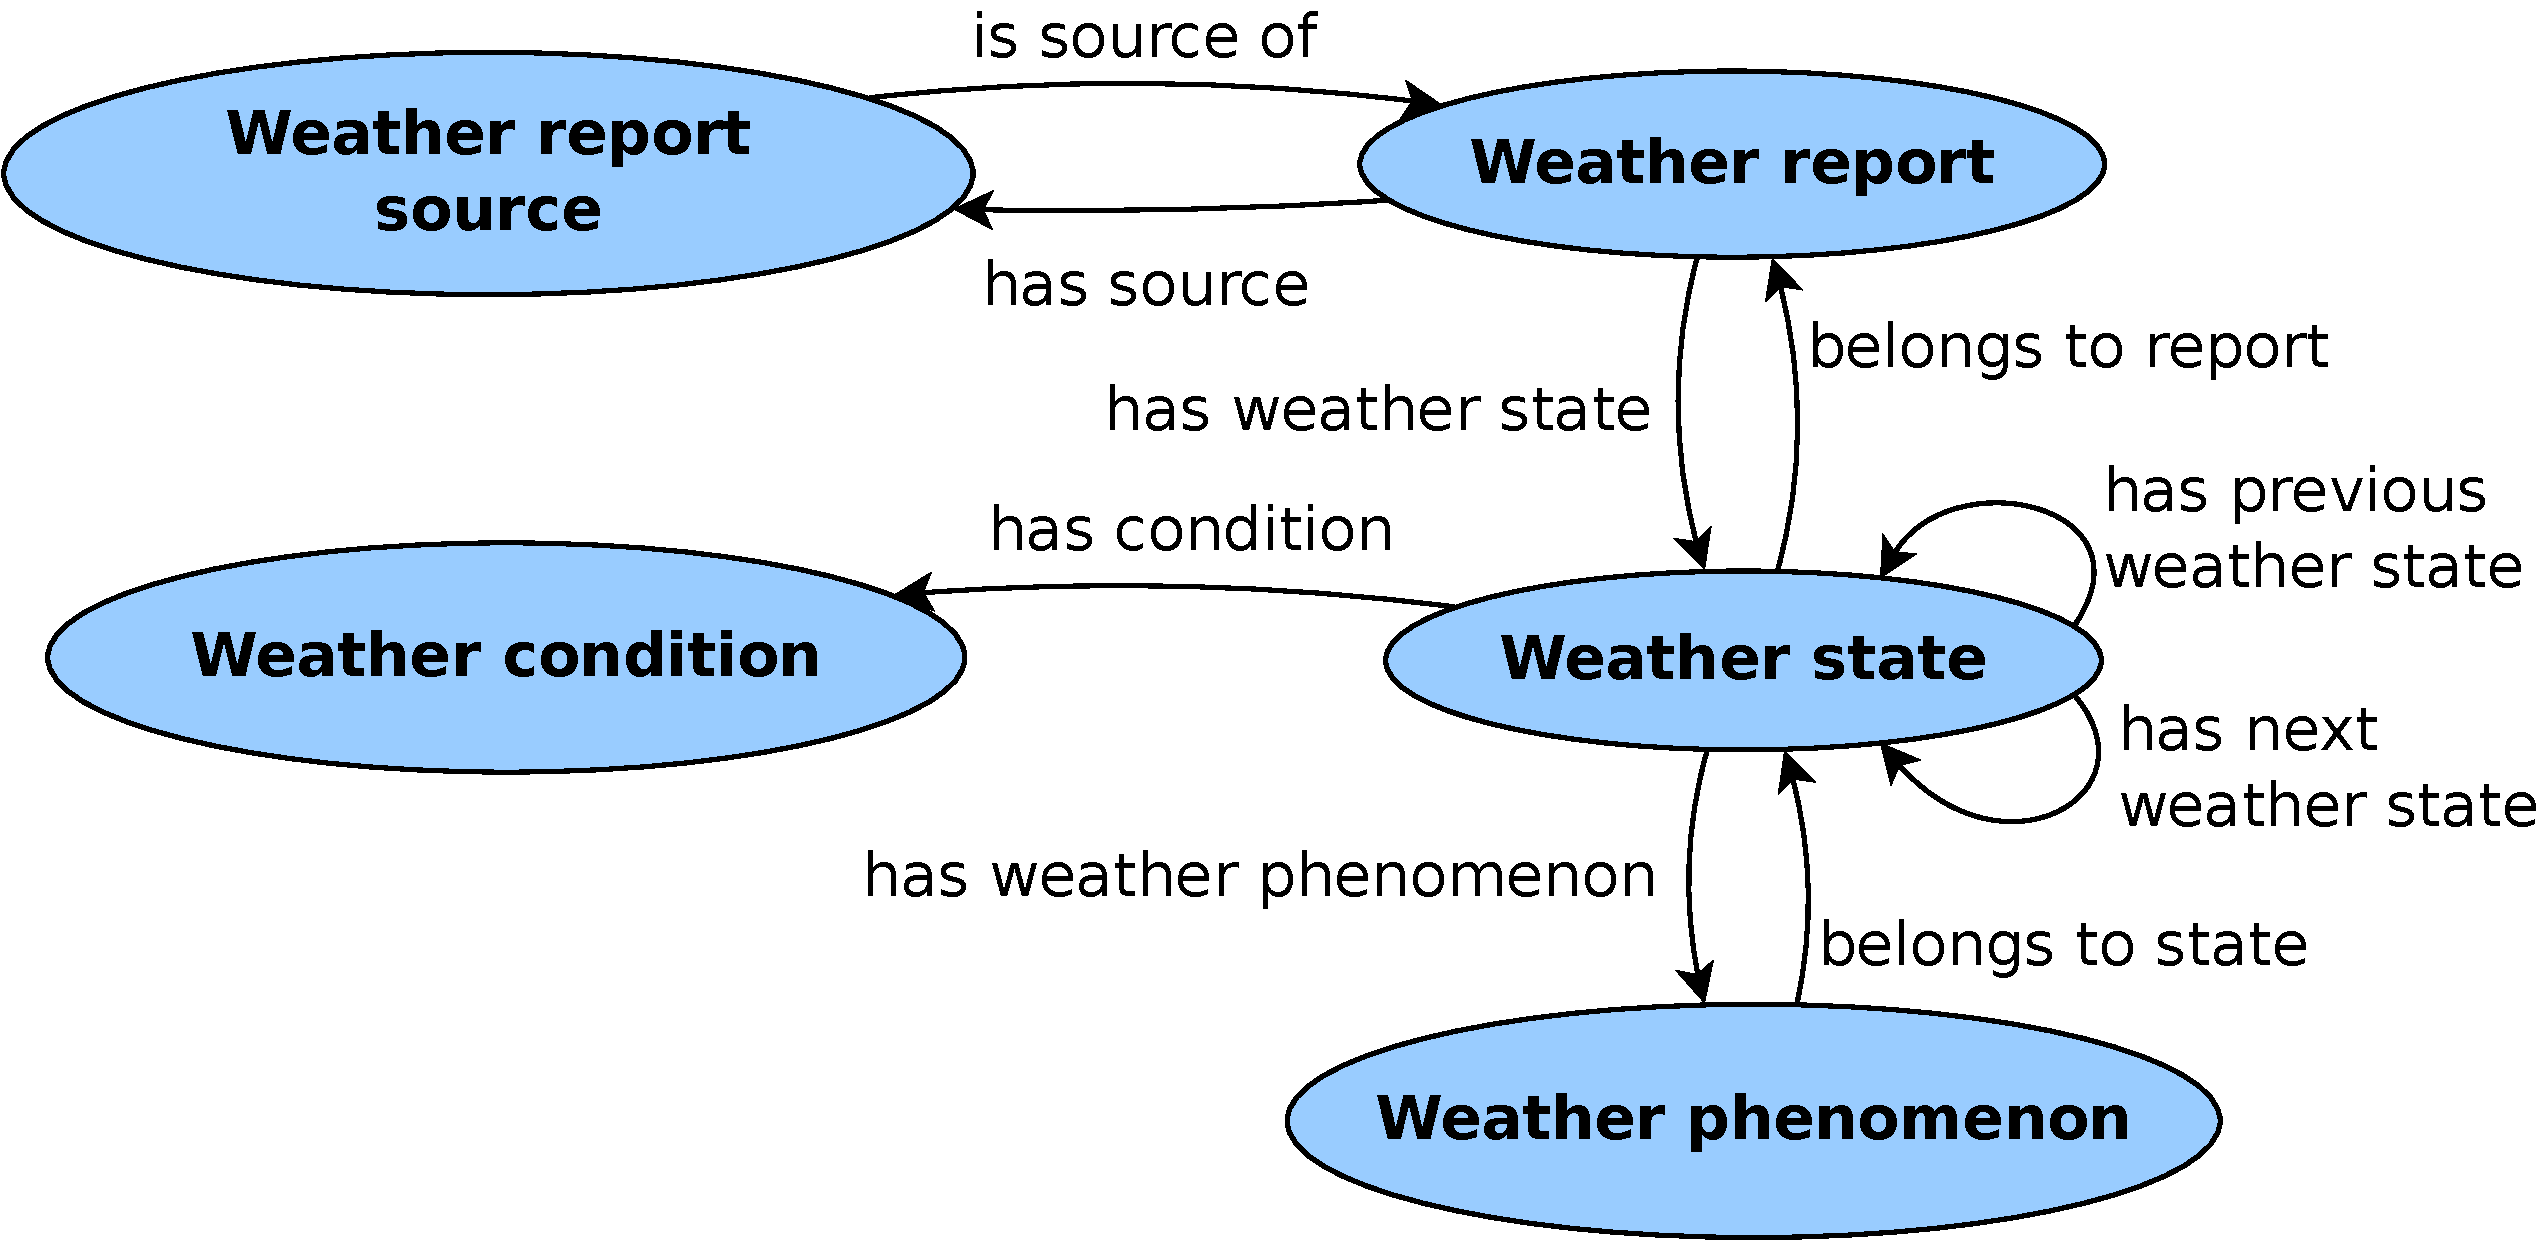
\includegraphics[width=.8\textwidth]{figures/diagrams/binary-relations.pdf}
  \caption{Binary relations diagram of \smarthomeweather}
  \label{fig:binary_relations}
\end{figure}

\subsection{Concept dictionaries}
\label{subsec:concept_dictionaries}

A \emph{Concept dictionary} lists all concepts together with their names, instances, class attributes, instance attributes, and relations. For the sake of clarity, this table is split up into several tables, one for each of the concept-classification trees from Section~\ref{sec:concept_classification_trees}.

The tables can be found in the appendix in Figure~\ref{fig:concept_dict1} (\Egls{weather condition}, \Egls{weather report}, and \Egls{weather source}) and Figure~\ref{fig:concept_dict2} (\Egls{weather phenomenon} and \Egls{weather state}). In these tables, sub-concepts having the same instances, class attributes, instance attributes and relations as their super-concepts are omitted. Furthermore, any columns that are not filled with any content in any row are omitted.

\subsection{Binary relations table}
\label{subsec:binary_relations_table}

The \emph{Binary relation table} specifies all relations from Section~\ref{subsec:binary_relations_diagram} in detail. This includes the relations' names, their source and target concepts, their maximum source cardinalities, and their inverse relations, if any. The table can be found in the appendix in Figure~\ref{fig:binary_relations_table}.

\subsection{Instance attributes table}
\label{subsec:instance_attributes_table}

An \emph{Instance attributes table} lists all instance attributes in \smarthomeweather together with the concept where they belong to, their value type and value range, the unit of measurement and their cardinality. The \emph{Instance attributes table} can be found in the appendix in Figure~\ref{fig:instance_attributes_table}.

The data types \emph{xsd:integer} and \emph{xsd:decimal} in the table refer to the types defined in \emph{\eacs{XML} Schema}\cite{xml-schema-datatypes}. For sake of simplicity, this table does not respect usage of the \emph{Measurements Unit Ontology} (\muo)~\cite{MUO}. In the ontology, all attributes listed below that belong to a sub-concept of \Egls{weather phenomenon} do not refer to a literal as stated here. Instead, they link to a blank node of type \emph{Quality value} which in turn has two attributes, one for the literal value (named \emph{numerical value}) and one for the unit (named \emph{measured in}). The type given in the table below is the type of the value the property \emph{numerical value} refers to. See Section~\ref{sec:ontology_imports} for details about the implementation of \muo in \smarthomeweather.

\subsection{Class attributes table}
\label{subsec:class_attributes_table}

Many concepts within the \smarthomeweather ontology define themselves to be specializations of other concepts (see Section~\ref{sec:concept_classification_trees} above). E.g. the concepts \Egls{very low pressure}, \Egls{low pressure}, \Egls{average pressure}, \Egls{high pressure} and \Egls{very high pressure} are all sub-concepts of \Egls{atmospheric pressure}. They all differ by the value of the instance attribute \egls{has pressure value} that every instance of \Egls{atmospheric pressure} has.

These concepts are summarised in the \emph{Class attributes table} in the appendix in Figure~\ref{fig:class_attributes_table1}, Figure~\ref{fig:class_attributes_table2}, and Figure~\ref{fig:class_attributes_table3}. As in the \emph{Instance attributes tables} in Section~\ref{subsec:instance_attributes_table}, this table does not respect the use of \muo; no units are specified.

\subsection{Instances table}
\label{subsec:instances_table}

The only pre-defined instances in \smarthomeweather are the instances of the concept \Egls{weather condition}. Their details can be found in the \emph{Instance table} in the appendix in Figure~\ref{fig:instances_table}.

\section{Integration}
\label{sec:integration}

One of the goals when designing an ontology is to reuse existing ontologies where possible\cite{reuse1,reuse2}. Chapter~\ref{ch:existing_work} sheds some light on a selection of existing ontologies around the domain of weather data. In the domain of \smarthomeweather, four areas have been identified where existing ontologies may be reused. These areas are location data (Section~\ref{subsec:location_ontologies}), measurement units (Section~\ref{subsec:unit_ontologies}), specifications of date and time (Section~\ref{subsec:date_ontologies}) and weather concepts (Section~\ref{sec:weather_ontologies}).

The following ontologies have been selected for the import into \smarthomeweather:
\begin{itemize}
  \item \emph{OWL-Time}\cite{owl-time} is used for specifying temporal data (for date and time of a \Egls{weather report}).
  \item The \emph{Basic Geo (WGS84 lat/long) Vocabulary}\cite{wgs84_vocabulary} is used for specifying the location a \Egls{weather report} if valid for.
  \item The \emph{Measurement Units Ontology}\cite{MUO} (\muo) is used to enrich measurement values of each \Egls{weather phenomenon} with a unit (e.g. temperature in \si{\celsius}, rain in \si{\milli\metre\per\hour}). Although \muo does come with a few shortcomings (see Section~\ref{sec:implementation}), it is the ontology that has been identified to be the the one that fits \smarthomeweather's requirements best.
  \item Unfortunately, no weather ontology has been identified that defines weather concepts in a way that suits \smarthomeweather's requirements. Hence, \smarthomeweather defines its own concepts and properties for the domain of weather data.
\end{itemize}

Section~\ref{sec:implementation} describes the reuse of the aforementioned ontologies within the \smarthomeweather ontology in detail.

\section{Implementation}
\label{sec:implementation}

% TODO reasoning

After exhaustive analysis and structuring in the previous sections, the step of implementing the ontology has become a straight-forward task.

The \smarthomeweather ontology is implemented in OWL using \protege 4.1 together with the \emph{Pellet} \eacs{OWL} 2 Reasoner. \emph{Pellet} includes \emph{Pellint}~\cite{pellint}, an ontology performance tool that uses a set of patterns to find possible performance problems in an \eacs{OWL} ontology. \emph{Pellint} has been used intensively to ensure it does not report any problems that could affect reasoning performance.

To ensure that the reasoning of all sub-concepts of \egls{weather phenomenon}, \egls{weather state} and \egls{weather report} works correctly, \emph{JUnit}~\cite{junit} is used (see Section~\ref{sec:importer_tests}). Every test case loads the \smarthomeweather ontology using the \emph{Jena framework}, adds appropriate individuals and checks using the \emph{Pellet reasoner} if reasoning is performed in the desired manner.

During implementation of \smarthomeweather in \eacs{OWL}, the identifiers of concepts, properties and instances in this document are modified by removing all space characters and concatenating all parts of the identifier using \emph{camel case}\cite{CamelCase}, e.g. \Egls{weather state} becomes \emph{WeatherState} and \egls{has start time} becomes \emph{hasStartTime}. Hence, in the \eacs{OWL} implementation, all identifiers match the regular expression \texttt{\textasciicircum[A-za-z0-9]+\$}.


\subsection{Imported ontologies}
\label{sec:ontology_imports}

During the implementation step, the ontologies listed in Section~\ref{sec:integration} need to be imported and integrated. Their use necessitates the application of certain patterns required by these ontologies.

\vspace{1em}

\emph{OWL-Time}\cite{owl-time} defines the concept \Egls{temporal entity} and its sub-concepts \Egls{instant} and \Egls{interval}, both having a self-explanatory name. The properties \egls{has start time}, \egls{has end time} and \egls{has observation time} of \egls{weather report} link to instances of \Egls{temporal entity}; however, only \egls{has observation time} is implemented to link an instance of \Egls{instant} to a \Egls{weather report}. For \egls{has start time} and \egls{has end time}, instances of \Egls{interval} are used. Such an instance represents the interval between the \egls{observation time} and the time the \Egls{weather report} is valid from/until (in hours). This simplifies reasoning of the sub-concepts of \Egls{weather report} which depend on the report's \egls{start time}; e.g. an instance of \emph{Forecast 1 hour weather report} can be defined as an instance of \Egls{weather report} having a \egls{start time} of \num{1} (hours).

Figure~\ref{fig:owl_time1} shows a \Egls{weather report} together with its with \egls{start time} and \egls{end time}; Figure~\ref{fig:owl_time2} displays a \Egls{weather report} together with its \egls{observation time}. The \emph{Time Zone Ontology} that comes with \emph{OWL-Time} is not used by \smarthomeweather. All times are given in \emph{UTC}.

\begin{figure}
  \centering
  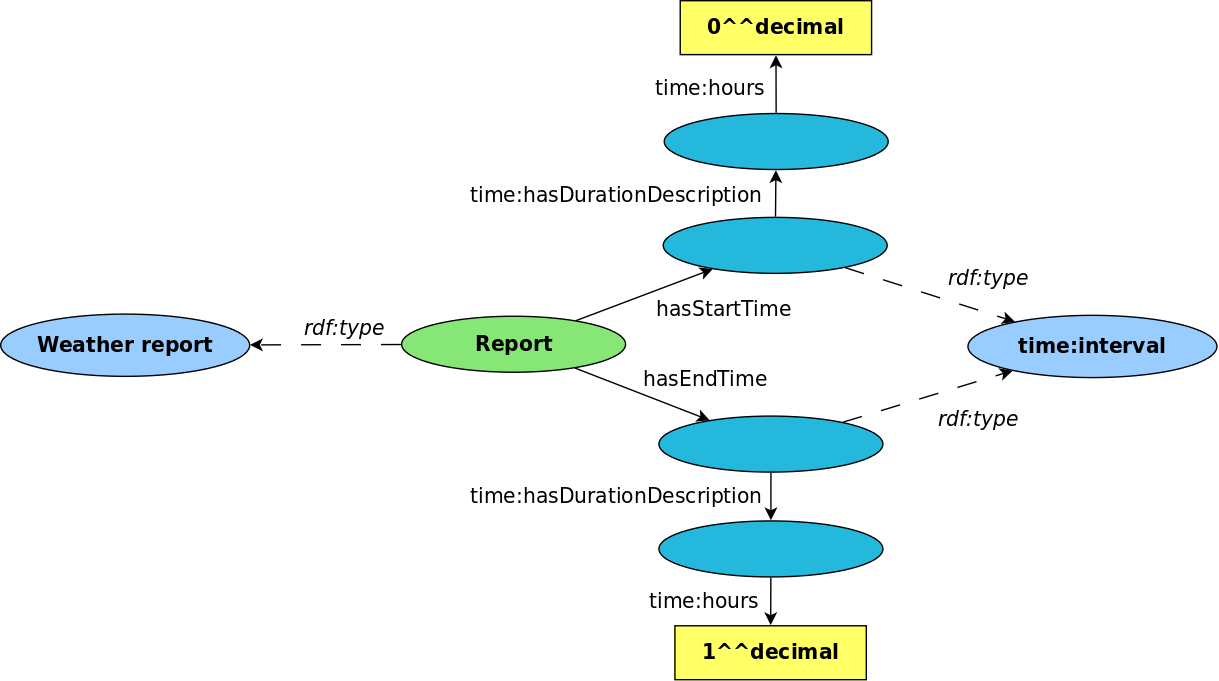
\includegraphics[width=\textwidth]{figures/diagrams/owl-time1.pdf}
  \caption{An instance of \Egls{current weather report} together with \egls{start time} and \egls{end time}}
  \label{fig:owl_time1}
\end{figure}

\begin{figure}
  \centering
  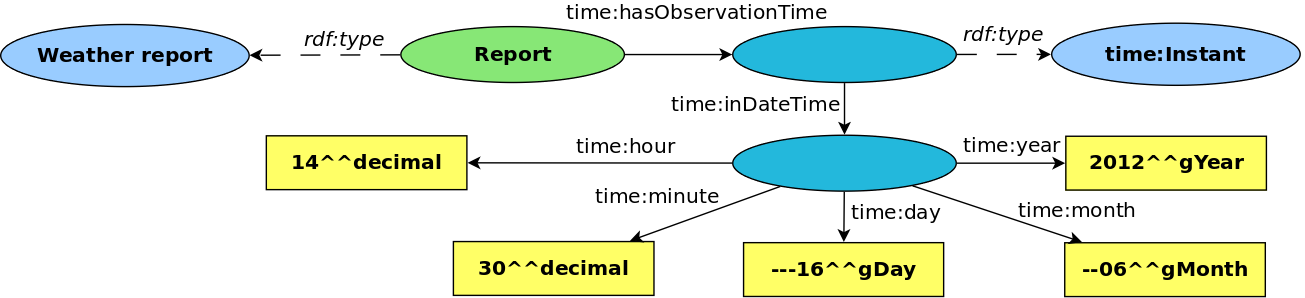
\includegraphics[width=\textwidth]{figures/diagrams/owl-time2.pdf}
  \caption{An instance of \Egls{weather report} together with its \egls{observation time} (\texttt{2012-06-16~14:30})}
  \label{fig:owl_time2}
\end{figure}

\vspace{1em}

Figure~\ref{fig:muo1} shows how an instance of \Egls{temperature} would be implemented if no ontology for units of measurements would be used. With the introduction of the \emph{Measurement Units Ontology} (\muo), the data property and the literal are removed; an object property that is a sub-property of \emph{Quality value} (which is defined by \muo) takes the place of the data property. It links to a blank node which in turn has two properties: \emph{Measured in} and \emph{numericalValue}. The property \emph{Measured in} is an object property that refers to the unit being used which is represented by an instance of \muo's concept \emph{Unit of measurement}. Using the data property \emph{numericalValue}, the literal is connected to the blank node. The resulting pattern is seen in Figure~\ref{fig:muo2}.

\begin{figure}
  \centering
  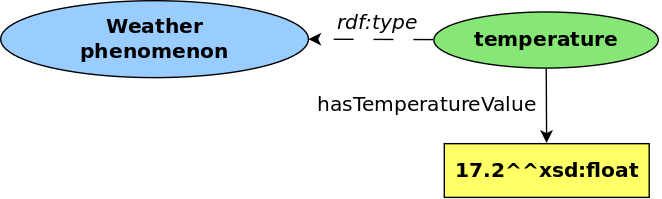
\includegraphics[width=.5\textwidth]{figures/diagrams/muo1.pdf}
  \caption{An instance of \Egls{temperature} together with the property \egls{has temperature value} representing a temperature of \SI{17.2}{\celsius} (without using a unit ontology)}
  \label{fig:muo1}
\end{figure}

\begin{figure}
  \centering
  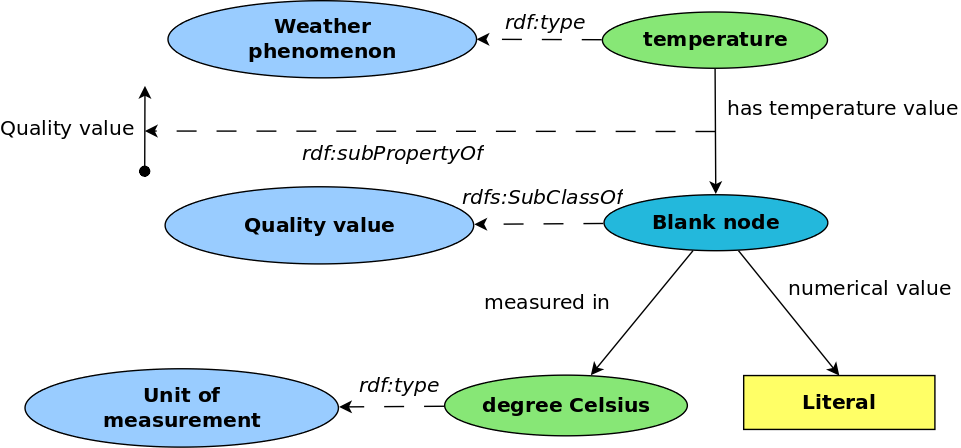
\includegraphics[width=.9\textwidth]{figures/diagrams/muo2.pdf}
  \caption{An instance of \Egls{temperature} together with the property \egls{has temperature value} representing a temperature of \SI{17.2}{\celsius} (using \muo)}
  \label{fig:muo2}
\end{figure}

\muo is an ontology that is easy to implement in an already-existing ontology. Its major drawback in the case of \smarthomeweather is that it affects reasoning time negatively. Repeated tests showed that reasoning time increased by about $30 \%$ when introducing \muo. However, the slowdown caused by \muo is accepted in favour of the usage of units of measurement.

\vspace{1em}

Figure~\ref{fig:owl_wgs84} shows how the \egls{location} of a \Egls{weather report} is encoded. % TODO mention geo ontology

\begin{figure}
  \centering
  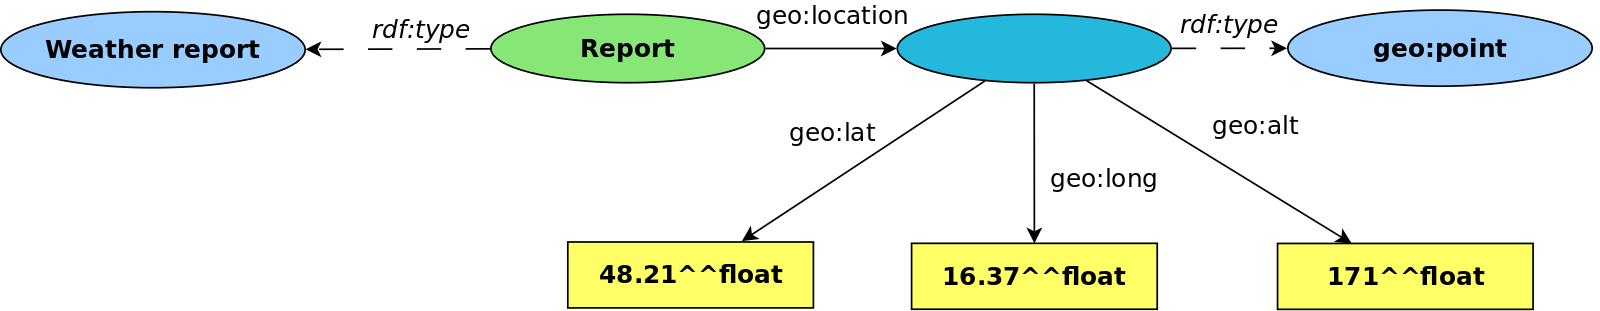
\includegraphics[width=\textwidth]{figures/diagrams/wgs84.pdf}
  \caption{An instance of \Egls{weather report} together with its \egls{location} (Vienna, Austria: N~\SI{48.21}{\degree}, E~\SI{16.37}{\degree}, \SI{171}{\metre} above \eacs{MSL}).}
  \label{fig:owl_wgs84}
\end{figure}

\section{Evaluation}
\label{sec:ontology_evaluation}

After completing the implementation step, this section evaluates \smarthomeweather regarding all non-functional requirements and functional requirements from Section~\ref{sec:weather_information} and the \emph{Ontology Requirements Specification Document} in Section~\ref{sec:ontology_specification}.

\subsection{Non-functional requirements}
\label{sec:evaluation_non_functional}

There are three non-functional requirements:

\begin{itemize}
  \item \textbf{Naming conventions}: All identifiers in \smarthomeweather follow the naming conventions stated in Section~\ref{sec:ontology_conventions}.
  \item \textbf{Documentation}: Due to following the \methontology approach, the ontology is well documented at every stage of development.
  \item \textbf{Usage of other ontologies}: \smarthomeweather imports the \emph{Basic Geo (WGS84 lat/long) Vocabulary}, \muo and \emph{OWL-Time}; no ontology has been found that satisfies the requirements of \smarthomeweather regarding concepts for weather data, thus \smarthomeweather defines its own concepts.
\end{itemize}

Thus, all non-functional requirements are met by \smarthomeweather.

\subsection{Functional requirements}
\label{sec:evaluation_functional}

\smarthomeweather meets its functional requirements if it provides answers to all competency questions. This section evaluates if answers are provided and how answers can be drawn from the ontology.

For the following questions, \smarthomeweather can give straight answers:
\begin{itemize}
  \item What is the current weather situation?
  \item What will the weather situation be in one hour, in two hours, …, in 24 hours?
  \item What is the current temperature, humidity, wind speed, …?
  \item What will be the temperature, humidity, wind speed, … in one hour, in two hours, …, in 24 hours?
  \item Does it rain?
\end{itemize}
To answer any of these questions, the relevant instance of \Egls{weather report} must be identified. Via the property \egls{has weather state}, an instance of \Egls{weather state} is connected to it; this instance has in turn an arbitrary number of \egls{has weather phenomenon} properties each linking to an instance of \Egls{weather phenomenon}. The information from these instances of \Egls{weather phenomenon} provide the desired answer.

However, there are questions that cannot be answered by \smarthomeweather as writing rules to infer answers would be too complicated in \eacs{OWL}:
\begin{itemize}
  \item Will the weather change? Will the temperature, humidity, … rise or fall?
  \item Do we need to irrigate the garden?
\end{itemize}

Furthermore, there are questions that cannot be answered using an \eacs{OWL} ontology due to the \emph{Open World Assumption}~\cite{open_world_assumption1}. For instance, an \eacs{OWL} reasoner cannot determine that some attribute value is the lowest one as it does not know whether there may be lower value it does not know anything about; the reasoner only knows about the presence of individuals and attribute values, but nothing about their absence.

\begin{itemize}
  \item What will be the minimum temperature, humidity, … over the next 24 hours? What about maximum values?
  \item Will it rain in the next hours? Will it rain today?
  \item Will there be sunshine today?
  \item Will there be severe weather?
  \item Will temperature drop/stay below \SI{0}{\celsius}?
  \item When can we open windows and when do we have to keep them shut?
  \item When do we need sun protection?
  \item When will it outside be colder than inside the house? When will it be warmer?
\end{itemize}

However, for each of the above competency questions, whether a direct answer can be given or not, \smarthomeweather can provide all available data; an external program (which is not limited by the \emph{Open World Assumption}) can access this data (e.g. using \eacs{SPARQL} queries) and generate an answer.

Hence, the ontology constructed in this chapter complies with its specification in Section~\ref{sec:ontology_specification}.

% TODO SPARQL queries/SWRL rules
